\documentclass[a4paper,14pt]{extreport}
\usepackage[left=1.5cm,right=1.5cm,
    top=1.5cm,bottom=2cm,bindingoffset=0cm]{geometry}
\usepackage{scrextend}
\usepackage[T1,T2A]{fontenc}
\usepackage[utf8]{inputenc}
\usepackage[english,russian,ukrainian]{babel}
\usepackage{tabularx}
\usepackage{amssymb}
\usepackage{color}
\usepackage{amsmath}
\usepackage{mathrsfs}
\usepackage{listings}
\usepackage{graphicx}
\graphicspath{ {./images/} }
\usepackage{lipsum}
\usepackage{xcolor}
\usepackage{hyperref}
\usepackage{tcolorbox}
\usepackage{tikz}
\usepackage{ulem}
\usepackage[framemethod=TikZ]{mdframed}
\usepackage{wrapfig,boxedminipage,lipsum}
\mdfdefinestyle{MyFrame}{%
linecolor=blue,outerlinewidth=2pt,roundcorner=20pt,innertopmargin=\baselineskip,innerbottommargin=\baselineskip,innerrightmargin=20pt,innerleftmargin=20pt,backgroundcolor=gray!50!white}
 \usepackage{csvsimple}
 \usepackage{supertabular}
\usepackage{pdflscape}
\usepackage{fancyvrb}
%\usepackage{comment}
\usepackage{array,tabularx}
\usepackage{colortbl}

\usepackage{varwidth}
\tcbuselibrary{skins}
\usepackage{fancybox}
\usepackage{spreadtab}
 % Цвета для гиперссылок
\definecolor{linkcolor}{HTML}{799B03} % цвет ссылок
\definecolor{urlcolor}{HTML}{799B03} % цвет гиперссылок


\usepackage{tikz}
\usepackage[framemethod=TikZ]{mdframed}
\usepackage{xcolor}
\usetikzlibrary{calc}
\makeatletter
\newlength{\mylength}
\xdef\CircleFactor{1.1}
\setlength\mylength{\dimexpr\f@size pt}
\newsavebox{\mybox}
\newcommand*\circled[2][draw=blue]{\savebox\mybox{\vbox{\vphantom{WL1/}#1}}\setlength\mylength{\dimexpr\CircleFactor\dimexpr\ht\mybox+\dp\mybox\relax\relax}\tikzset{mystyle/.style={circle,#1,minimum height={\mylength}}}
\tikz[baseline=(char.base)]
\node[mystyle] (char) {#2};}
\makeatother

\definecolor{ggreen}{rgb}{0.4,1,0}
\definecolor{rred}{rgb}{1,0.1,0.1}
\definecolor{amber}{rgb}{1.0, 0.75, 0.0}
\definecolor{babyblue}{rgb}{0.54, 0.81, 0.94}
\definecolor{amethyst}{rgb}{0.6, 0.4, 0.8}

\usepackage{float}
\usepackage{wrapfig}
\usepackage{framed}
%for nice Code{
\lstdefinestyle{customc}{
  belowcaptionskip=1\baselineskip,
  breaklines=true,
  frame=L,
  xleftmargin=\parindent,
  language=C,
  showstringspaces=false,
  basicstyle=\small\ttfamily,
  keywordstyle=\bfseries\color{green!40!black},
  commentstyle=\itshape\color{purple!40!black},
  identifierstyle=\color{blue},
  stringstyle=\color{orange},
}
\lstset{escapechar=@,style=customc}
%
  % Цвета для гиперссылок
  \definecolor{linkcolor}{rgb}{0, 0.72, 0.92} % цвет ссылок
  \definecolor{urlcolor}{rgb}{0.0, 0.0, 1.0}% цвет гиперссылок
  \hypersetup{pdfstartview=FitH,  linkcolor=linkcolor,urlcolor=urlcolor,citecolor=red, colorlinks=true}



\begin{document}
\pagecolor{white}

%----------------------------------------1
\newtcbox{\xmybox}[1][red]{on line, arc=7pt,colback=#1!10!white,colframe=#1!50!black, before upper={\rule[-3pt]{0pt}{10pt}},boxrule=1pt, boxsep=0pt,left=6pt,right=6pt,top=2pt,bottom=2pt}

\begin{titlepage}
  \begin{center}
    \large
    Національний технічний університет України \\ "Київський політехнічний інститут імені Ігоря Сікорського"


    Факультет Електроніки

    Кафедра мікроелектроніки
    \vfill

    \textsc{ЗВІТ}\\

    {\Large Про виконання лабораторної роботи №1\\
      з дисципліни: «ФУНКЦІОНАЛЬНА ЕЛЕКТРОНІКА»\\[1cm]

        “Дослідження статичних характеристик оптронів”


    }
  \bigskip
\end{center}
\vfill

\newlength{\ML}
\settowidth{\ML}{«\underline{\hspace{0.4cm}}» \underline{\hspace{2cm}}}
\hfill
\begin{minipage}{1\textwidth}
Виконавець:\\
Студент 4-го курсу \hspace{4cm} $\underset{\text{(підпис)}}{\underline{\hspace{0.2\textwidth}}}$  \hspace{1cm}А.\,С.~Мнацаканов\\
\vspace{1cm}

Перевірив: \hspace{6.1cm} $\underset{\text{(підпис)}}{\underline{\hspace{0.2\textwidth}}}$  \hspace{1cm}С.\,В.~Малюта\\

\end{minipage}

\vfill

\begin{center}
2021
\end{center}
\end{titlepage}



\newpage
\setcounter{page}{2}
Мета роботи -- дослiдження динамiчних характеристик оптронiв та функцiональних при-
строїв на їх основi.\\

Порядок виконання роботи\\ 
\begin{enumerate}

\item Зiбрати схему для дослiдження динамiчних характеристик дiодного оптро-
на, який складається з кремнiєвого фотодiода та червоного свiтлодiода.
\item  На вхiд свiтлодiода подати перiодичний iмпульсний сигнал вiд генератора
(параметри задаються викладачем).
\item  На двохпроменевому осцилографi зняти форму сигналу з фотодiода. Визна-
чити значення часу включення та часу виключення оптрона по передньому
та задньому фронтах iмпульсу на рiвнi 0.1 та 0.9 амплiтудного значення,
тривалiсть вихiдного iмпульсу та час затримки по рiвню 0.5 амплiтудного
значення.
\item  Визначити залежнiсть динамiчних параметрiв вiд амплiтуди вхiдного iм-
пульсу (дiапазон задається викладачем).
\item  Визначити залежнiсть динамiчних параметрiв вiд тривалостi вхiдного iм-
пульсу (дiапазон задається викладачем).
\item  Вимкнути генератор та осцилограф.
\end{enumerate}

   \begin{figure}[h]
    \center{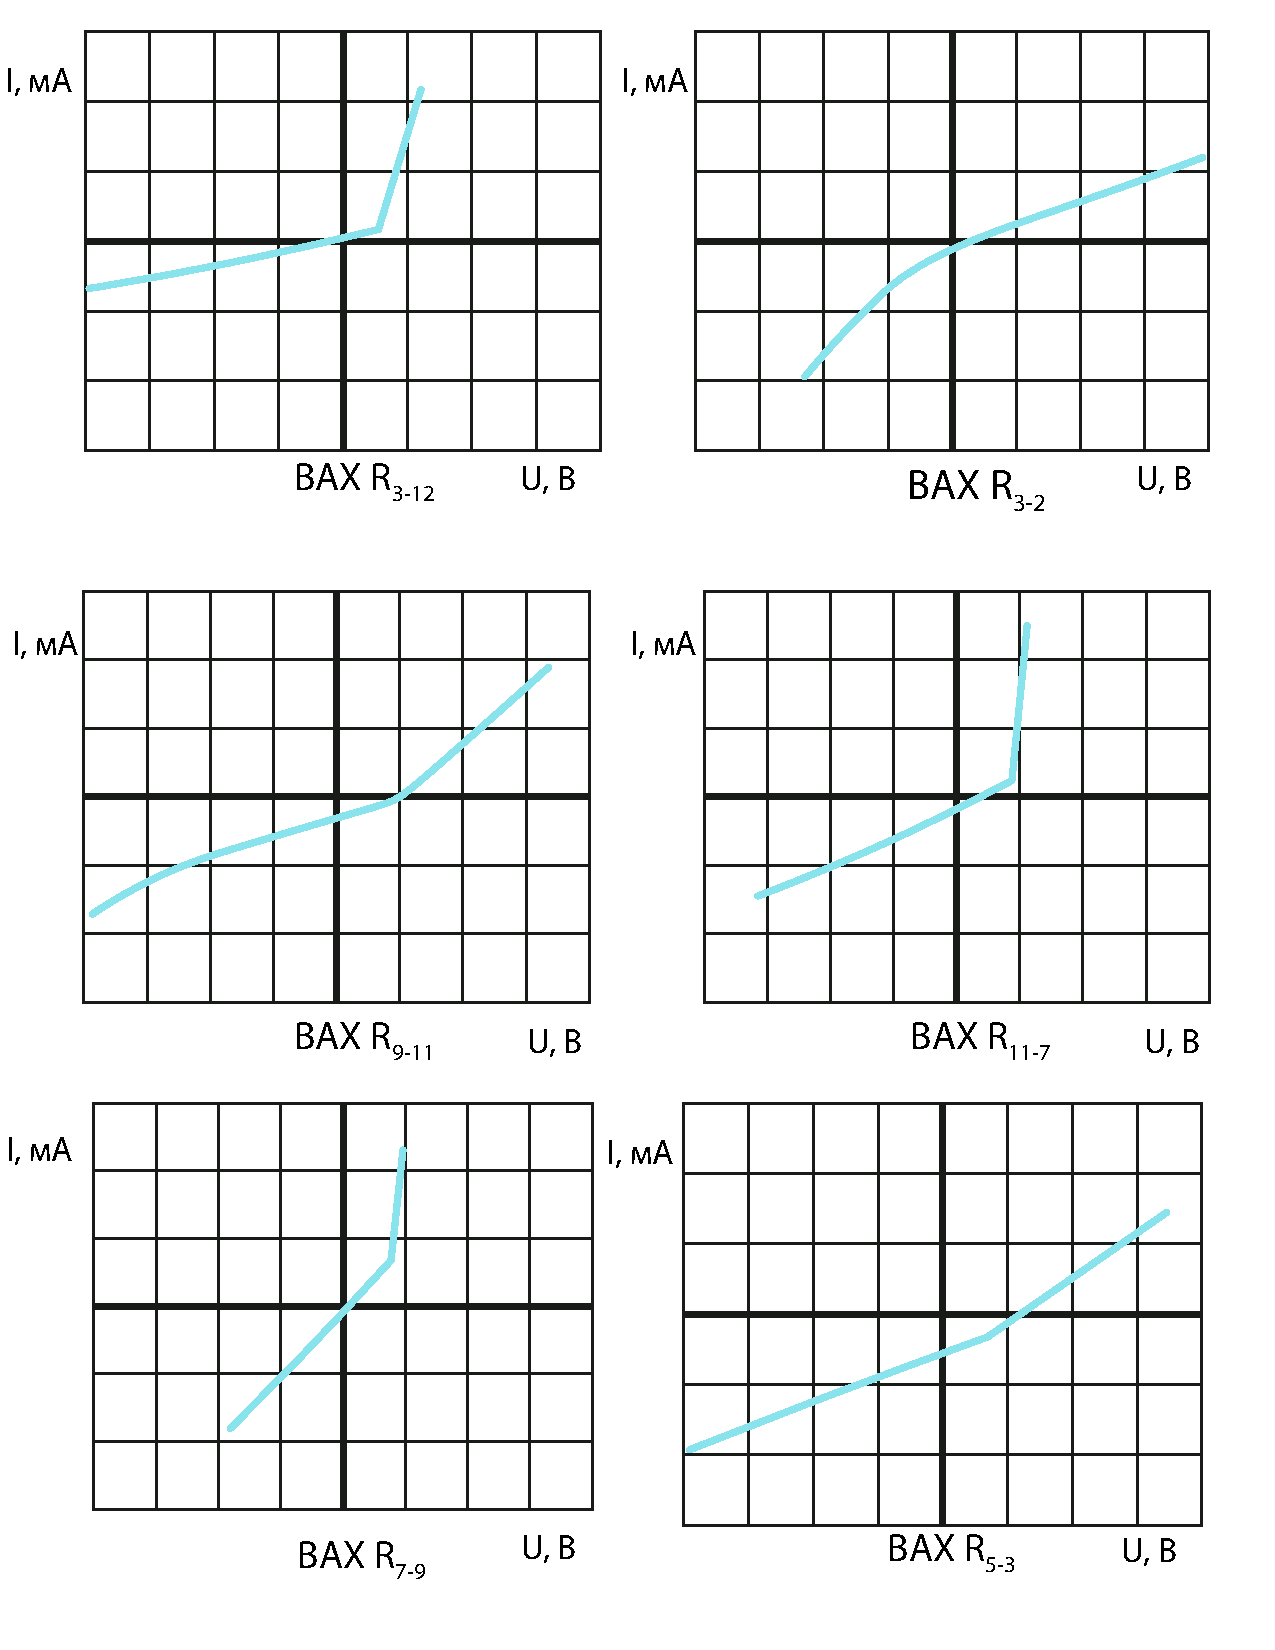
\includegraphics[width=0.7\linewidth]{111.png}}
    \caption{ Макет для дослiдження динамiчних характеристик оптронiв}
    \label{ris2}
  \end{figure}


\begin{center}
Результати вимiрювань
\end{center}


  \begin{figure}[h!]
  \center{Табл. 1: Вимiрянi динамiчнi характеристики оптронiв.
    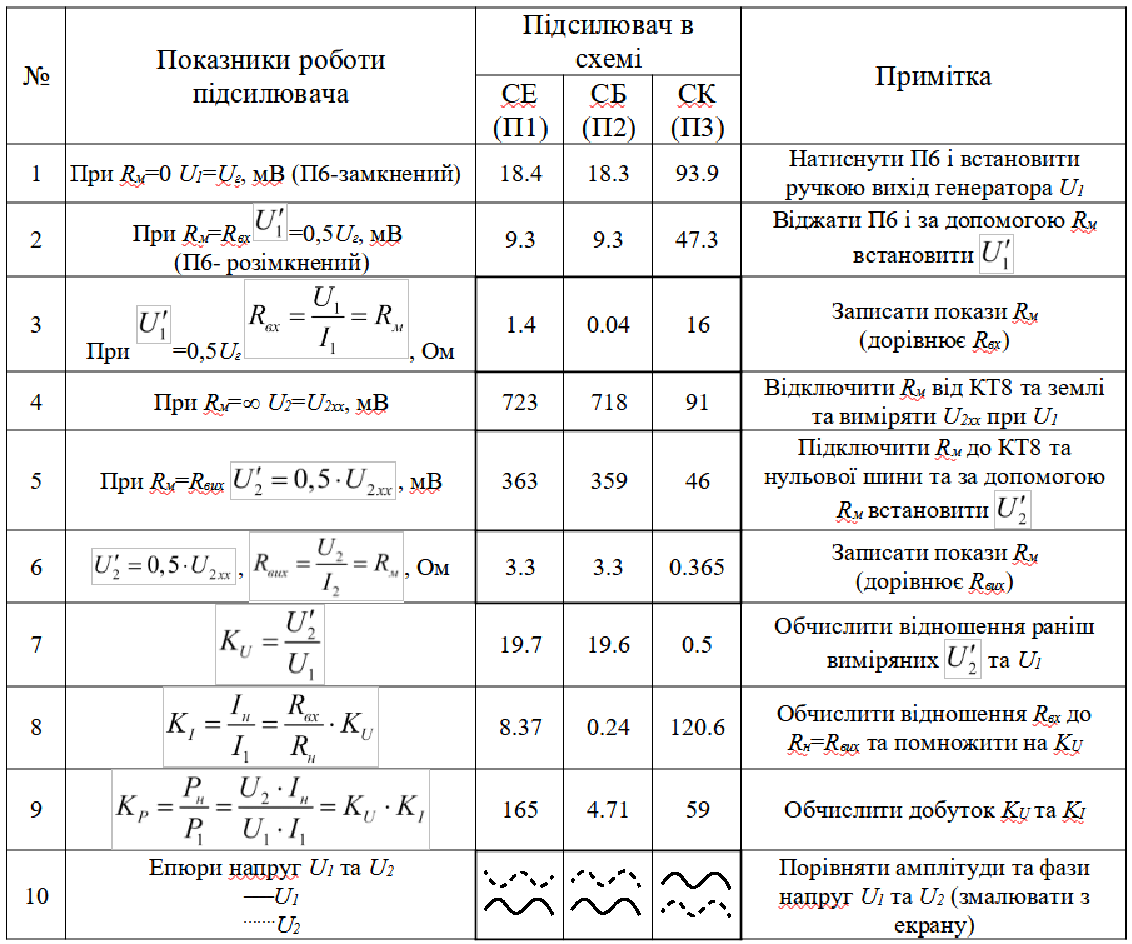
\includegraphics[width=0.4\linewidth]{t1.png}}
     
  \end{figure}


\begin{center}
Графiки
\end{center}


 \begin{figure}[h!]
    \center{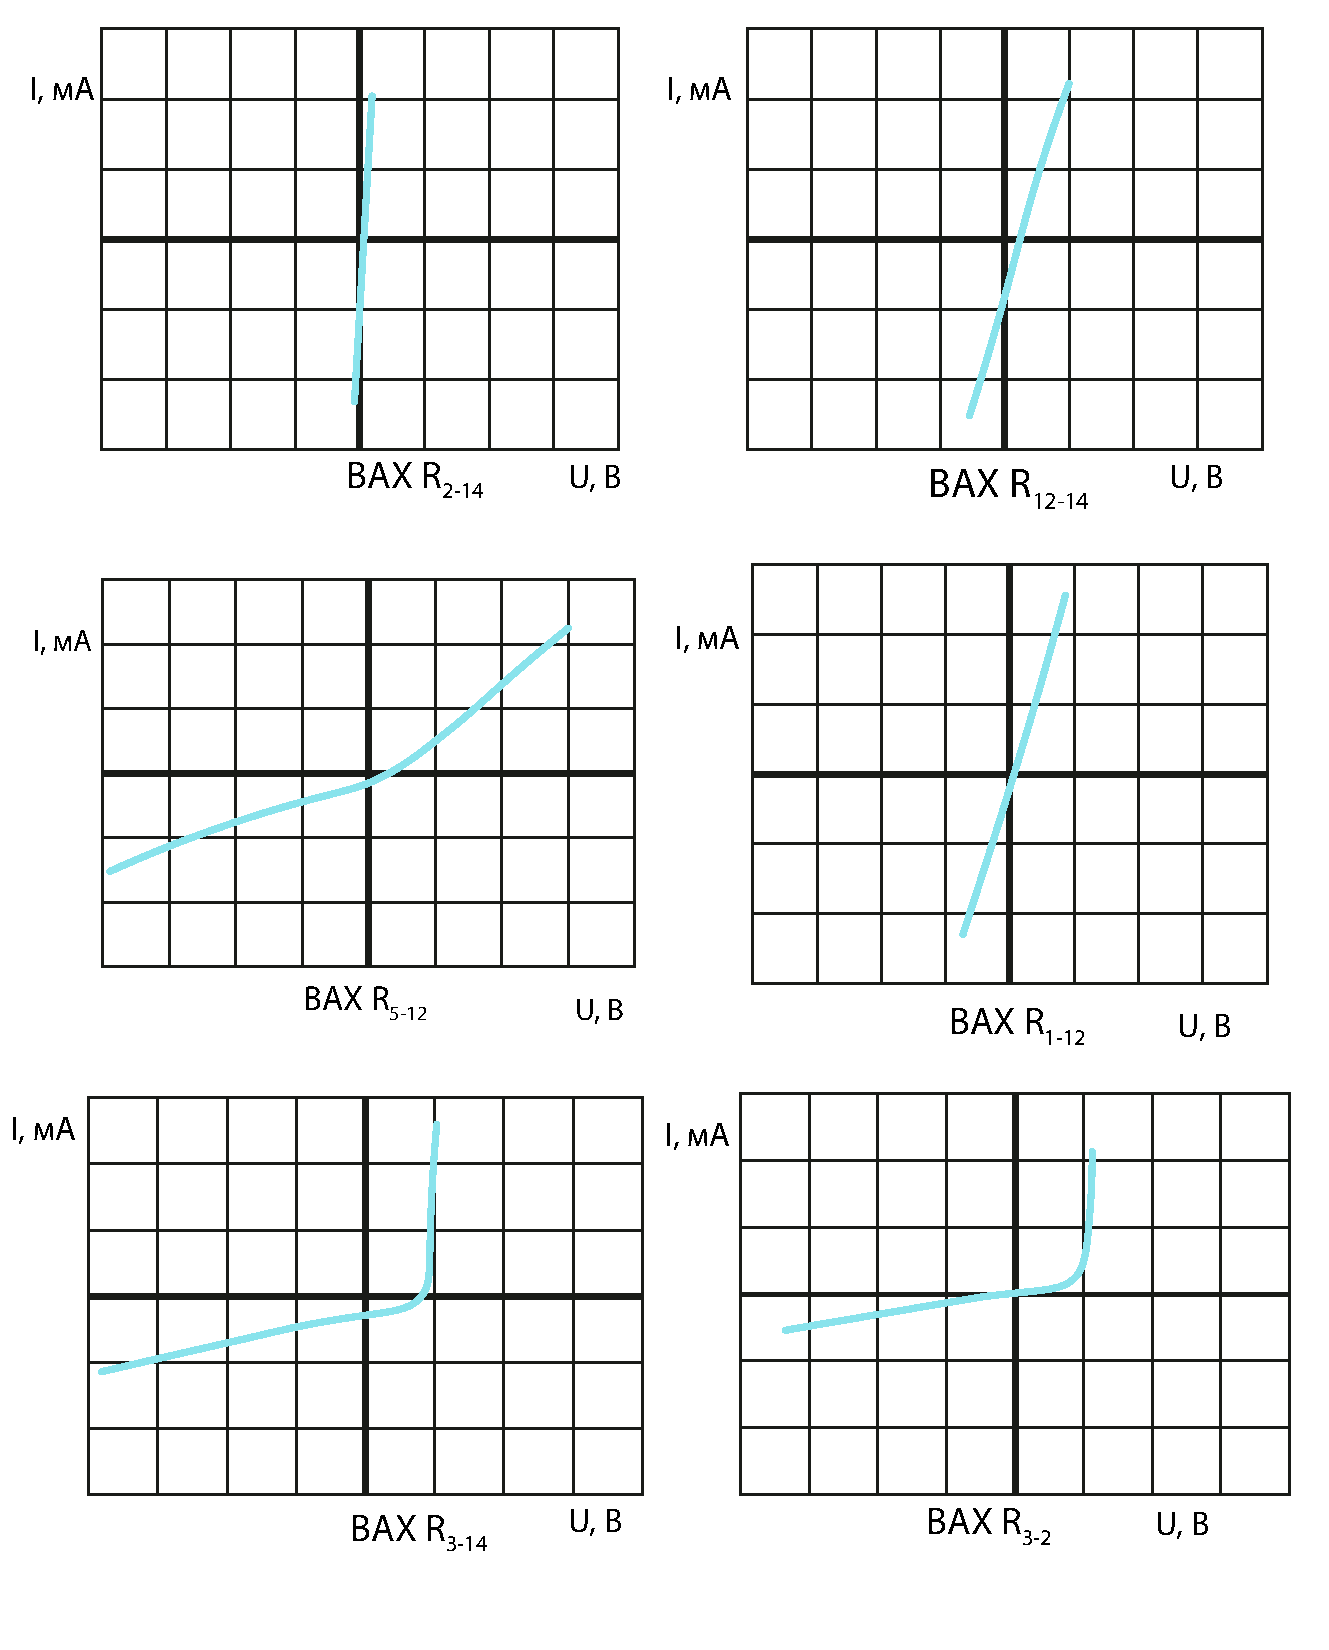
\includegraphics[width=0.7\linewidth]{222.png}}
    \caption{ Залежнiсть переднього фронту вiд амплiтуди вхiдного сигналу.}
    \label{ris2}
  \end{figure}


 \begin{figure}[h!]
    \center{\includegraphics[width=0.7\linewidth]{333.png}}
    \caption{  Залежнiсть заднього фронту вiд амплiтуди вхiдного сигналу.}
    \label{ris2}
  \end{figure}





 \begin{figure}[h!]
    \center{\includegraphics[width=0.7\linewidth]{444.png}}
    \caption{  Залежнiсть тривалостi iмпульсу вiд амплiтуди вхiдного сигналу.}
    \label{ris2}
  \end{figure}
\clearpage 
\begin{center}
Висновок
\end{center}

Проаналiзуємо отриманi залежностi. З рис.2 ми бачимо, що хоч експеримен-
тальнi точки трохи «плавають», тенденцiя зрозумiла: при пiдвищеннi амплiтуди
вхiдного сигналу переднiй фронт зменшується. Я б не сказав, що експерименталь-
нi данi взагалi неточнi, оскiльки маючи початкову амплiтуду 2 В та збiльшивши
ї ї в 2 рази, ми отримали зменшення тривалостi переднього фронту на порядок
(0,03 мс при 2 В та 0,004 при 4 В) - а це суттєво.\\ 

Натомiсть що ми бачимо на залежностi заднього фронту та тривалостi вихi-
дного iмпульсу (рис.3 та рис.4 вiдповiдно) - з першого погляду незрозумiлi плава-
ючi значення з деякою перiодичнiстю. Проте, якщо вгледiтись на шкалу
 y
 й при-
кинути розмах значень, то вiн виявиться досить малим - для рис.3 $t_{10,max}$
 = 0.36
мс,
 $t_{10,max}$ = 0.28
 мс, рiзниця
 $\triangle t_{10}$ = 0,08
 мс; для рис.2
 $t_{\text{трив},max}$ = 0,64
 мс,
tтрив,min = 0,60 мс, рiзниця $\triangle$tтрив = 0,04 мс. Тобто розкид значень складає всього
сотi долi.\\ 

Звичайно це можна списати на неточнiсть приладу або людський фактор,
проте, якщо дивитись в укрупненому масштабi на рис.3 та рис.4 з вiдображення
по осi y  значень що вiдрiзняються на порядок, то ми б отримали пряму лiнiю.\\ 

Отже пiдсумовуючи, при збiльшеннi амлiтуди вхiдного сигналу, переднiй
фронт зменшується, заднiй фронт та тривалiсть вихiдного iмпульсу залишаються
сталими.


 \begin{figure}[h!]
    \center{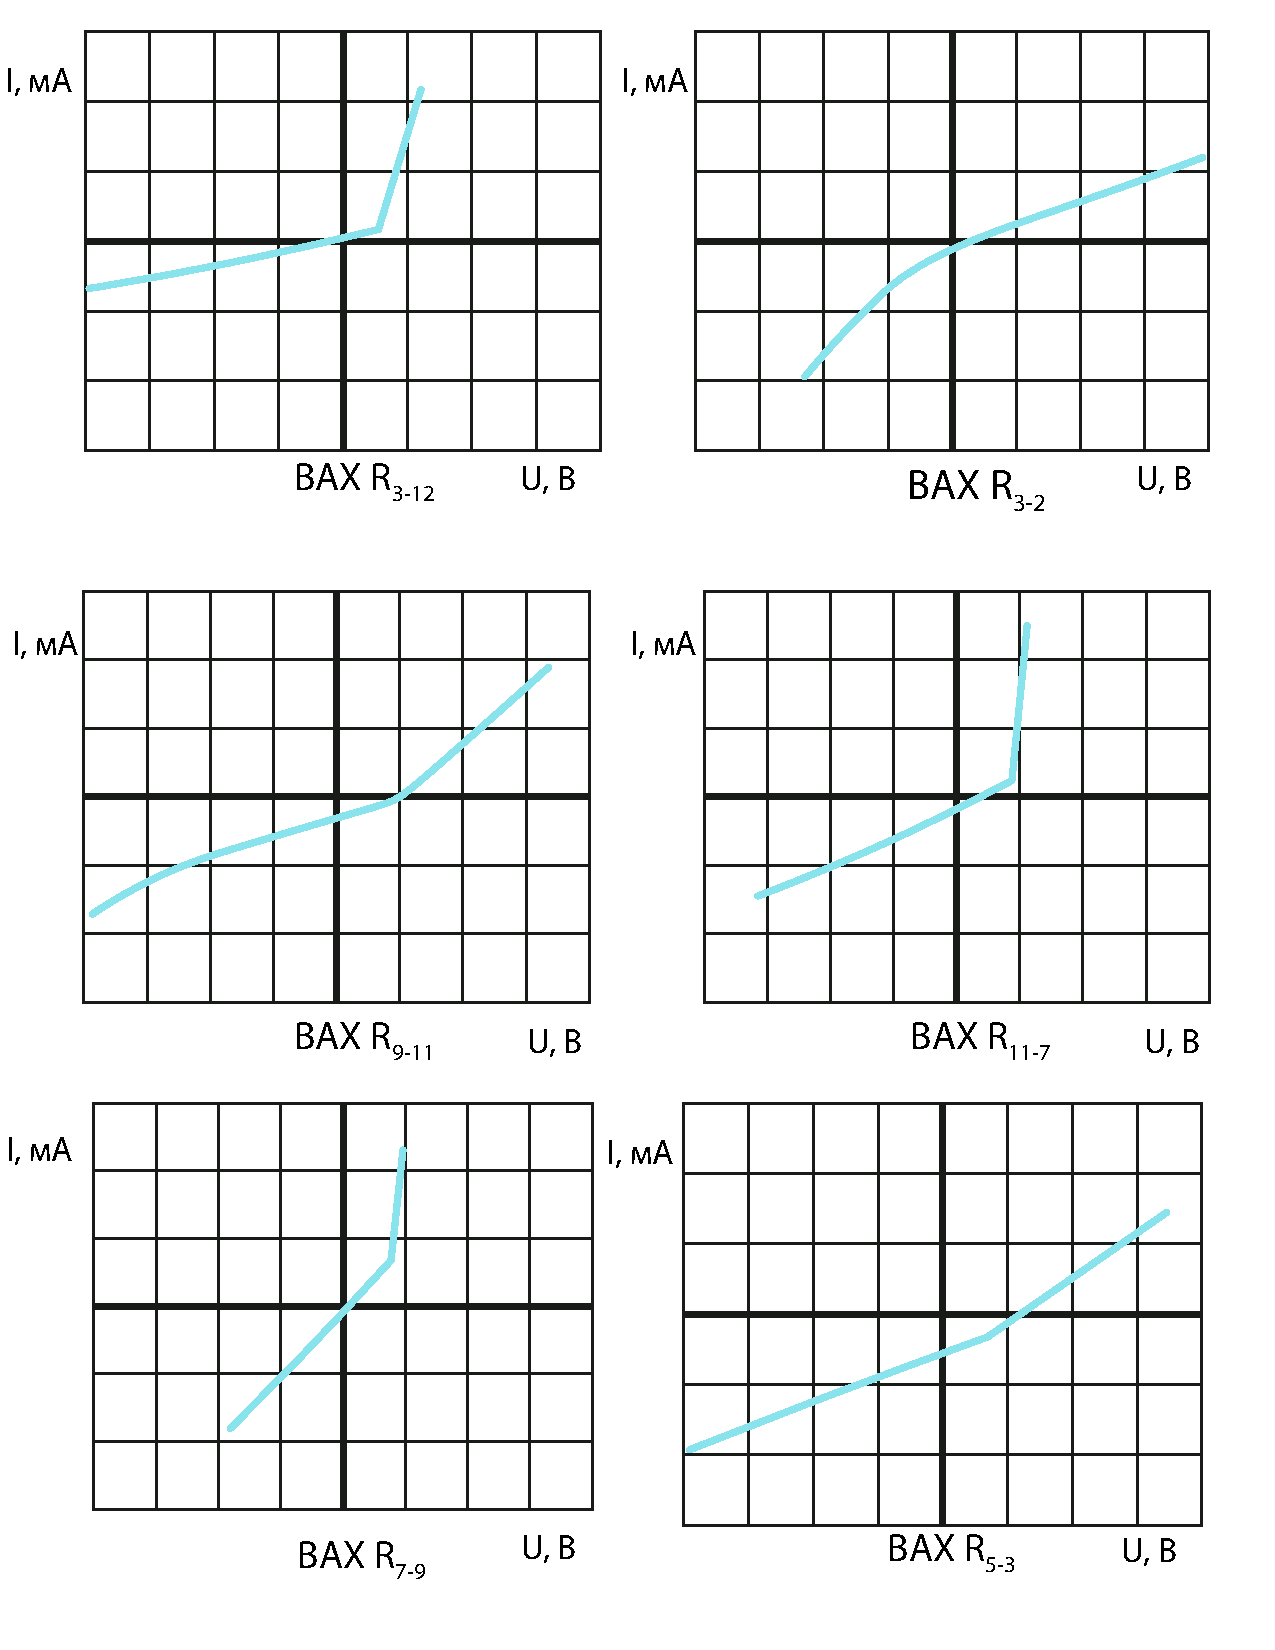
\includegraphics[width=0.7\linewidth]{111.jpg}}
     
  \end{figure}





\end{document}